\documentclass{beamer}
\usepackage{listings}

\begin{document}

\title[git]
{A short introduction to version control with Git}
\subtitle{Git - You'll never learn it all!}
\author[Blundell]
{Benjamin ~Blundell\inst{1}}
\institute[ITS Research, QMUL]
{
  \inst{1}
  ITS Research\\
  Queen Mary University of London
 }
\date[2016]
{CIS Software Engineering Day, 2016}
\subject{Computer Science}

% Slides
% Title
\frame{\titlepage}


% Introduction
\begin{frame}
  \frametitle{Introduction}
  
  \begin{block}{Me}
    \begin{itemize}  
      \item b.blundell@qmul.ac.uk 
      \item ITS Research - writing programs for scientists and artists.
      \item Helping people with their HPC problems.
      \item Previously ran small company building graphics-type things
      \item I write stuff at www.section9.co.uk
      \item I use Git everyday
    \end{itemize}
  \end{block}

\end{frame}


% What is it?
\begin{frame}
  \frametitle{What is it?}

  \begin{block}{What is git?}
    \begin{itemize}  
      \item Version control system developed for the Linux Kernel. 
      \item Distributed as opposed to centralised.
      \item A suite of many, many small tools.
    \end{itemize}
  \end{block}

  \begin{block}{What is github?}
    \begin{itemize}  
      \item Git, but on the internets.
      \item User-friendly interface including visualisations.
      \item A social network of sorts.
    \end{itemize}
  \end{block}

\end{frame}

% Why?
\begin{frame}
  \frametitle{How will Git help me right now?}

  \begin{block}{Advantages to version control}
    \begin{itemize}  
      \item Backing up your work.
      \item Undo-ing changes you've made.
      \item Sharing work with others.
    \end{itemize}
  \end{block}

  \begin{block}{Advantages to github}
    \begin{itemize}  
      \item Collaboration (showing off?).
      \item Off-site backup of code.
      \item Public accountability.
      \item Open-source contribution.
      \item A place to put all my slides so you can get them easily.
    \end{itemize}
  \end{block}

\end{frame}

% Resources
\begin{frame}
  \frametitle{Resources}

  \begin{block}{Reference material}
    \begin{itemize}
      \item https://git-scm.com/doc
      \item https://git-scm.com/book/en/v2
      \item man pages for git
    \end{itemize}
  \end{block}

  \begin{block}{Tutorials}
    \begin{itemize}  
      \item https://try.github.io/
      \item http://gitreal.codeschool.com/
    \end{itemize}
  \end{block}

  \begin{block}{Software}
   \begin{itemize}  
      \item Git for Windows.
      \item TortoiseGit.
      \item Git is built into Visual Studio and others.
    \end{itemize}

  \end{block}
\end{frame}

% Basic Commands
\begin{frame}[fragile]
  \frametitle{Lets begin}

  \begin{lstlisting}[caption=clone a repository] 
  git clone https://github.com/QMUL/ntlmgen
  git log
  git status
  \end{lstlisting}

  \begin{lstlisting}[caption=create a new repository] 
  git init 
  \end{lstlisting}

\end{frame}


% Changes
\begin{frame}[fragile]
  \frametitle{Making changes}
  
  \begin{lstlisting}[caption=Making changes] 
  git status
  git add licence.txt
  git status
  git commit -a -m "Altered readme \
   and added a licence"
  \end{lstlisting}

\end{frame}

% Branching

\begin{frame}[fragile]
  \frametitle{Branching out}
  
  \begin{lstlisting}[caption=Branching] 
  git branch alpha
  git checkout alpha
  git branch
  git commit -a -m "altered ntlmgen"
  git push origin alpha
  \end{lstlisting}

\end{frame}

% merging

\begin{frame}[fragile]
  \frametitle{Merging}
  
  \begin{lstlisting}[caption=Merging] 
  git checkout master
  git merge alpha
  git status
  git branch -d alpha
  \end{lstlisting}

\end{frame}


% recovery

\begin{frame}[fragile]
  \frametitle{Undoing mistakes}
  
  \begin{lstlisting}[caption=Hard Reset] 
  git reset --hard HEAD
  \end{lstlisting}

\end{frame}


% remotes

\begin{frame}[fragile]
  \frametitle{Remotes}
  
  \begin{lstlisting}[caption=Remotes] 
  git remote show
  git remote show origin
  git push origin master
  \end{lstlisting}

\end{frame}


\begin{frame}
  \frametitle{Time for a break}
 
  \begin{itemize} 
    \item Practical session to follow 
  \end{itemize}
 
\end{frame}


% Advanced Topics

% stashing

\begin{frame}[fragile]
  \frametitle{Stashing}
  Sometimes you want to temporarily store changes and come back to them later without commiting.

  \begin{lstlisting}[caption=stashing] 
  git stash
  git status
  git stash list
  git stash apply
  \end{lstlisting}

\end{frame}

% rebasing

\begin{frame}
  \frametitle{rebasing}
    Rebasing, in some ways, is another way to perform a merge (amongst other things). It *replays* changes on-top of a common ancestor.


  \begin{block}{example with merging}
    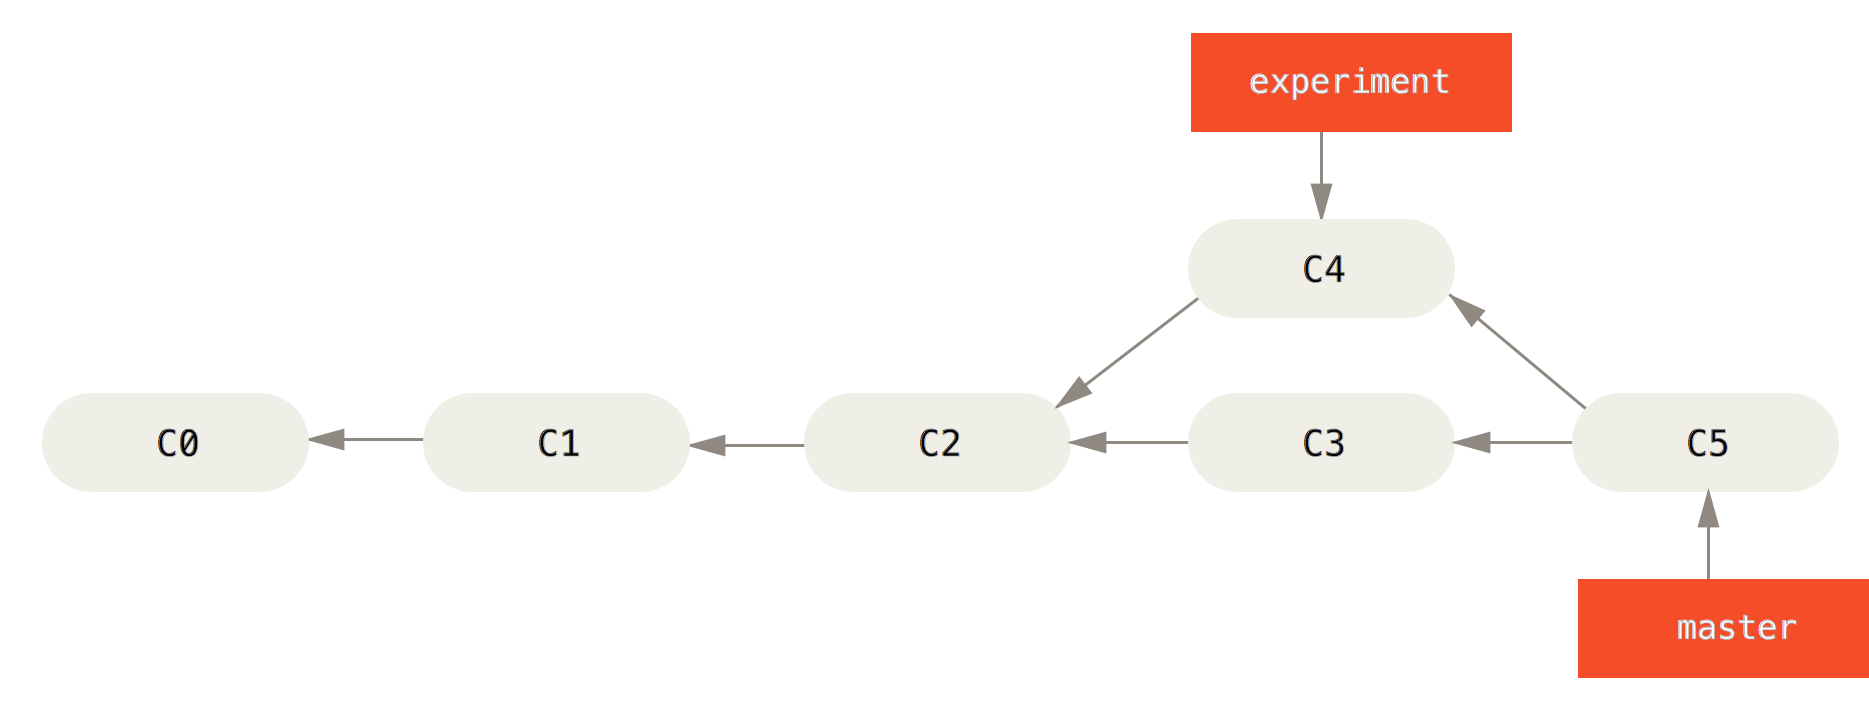
\includegraphics[height=3cm]{basic-rebase-2.png}
  \end{block}

\end{frame}

\begin{frame}[fragile]
  \frametitle{rebasing 2}
  
  \begin{lstlisting}[caption=rebase] 
   git checkout experiment
   git rebase master
  \end{lstlisting}

  \begin{block}{example with a rebase}
    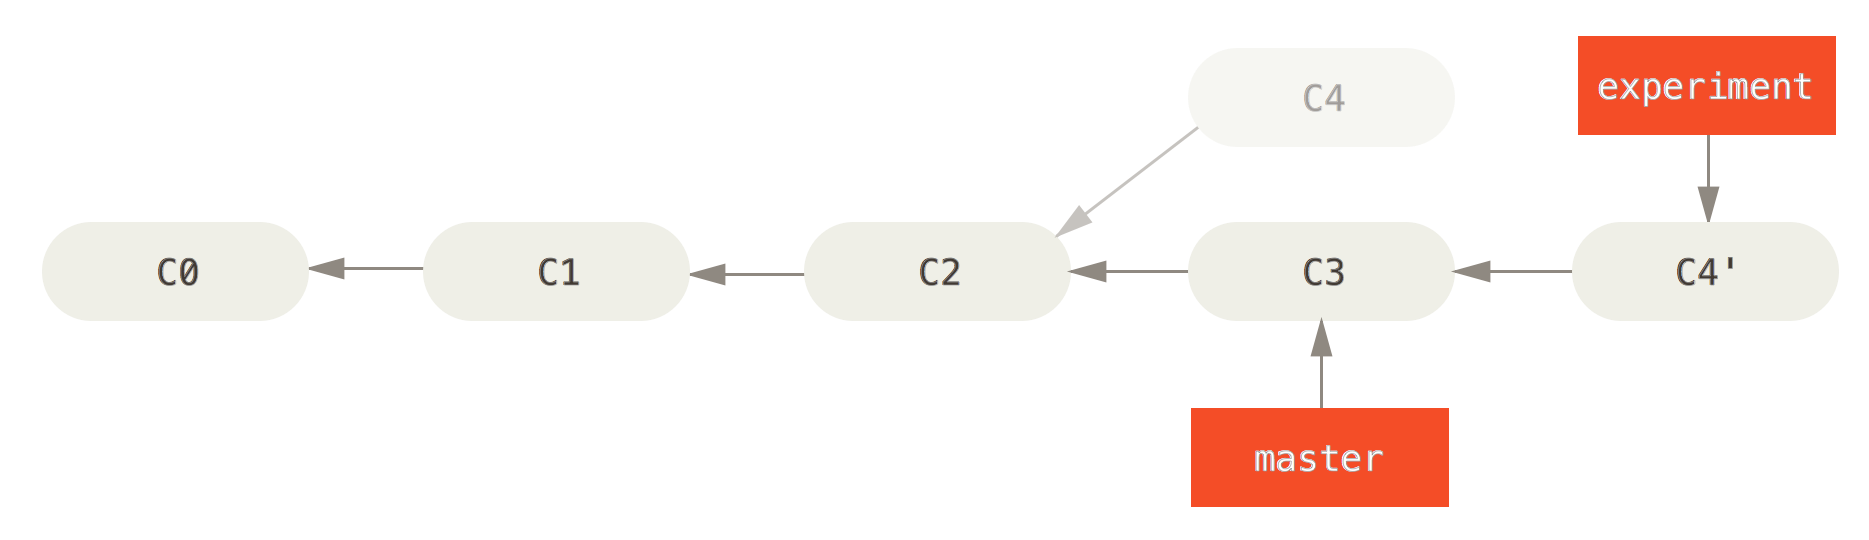
\includegraphics[height=3cm]{basic-rebase-3.png}
  \end{block}

\end{frame}

\begin{frame}[fragile]
  \frametitle{rebasing 3}
  
  \begin{lstlisting}[caption=rebase] 
    git checkout master
    git merge experiment
  \end{lstlisting}

  \begin{block}{example with a rebase}
    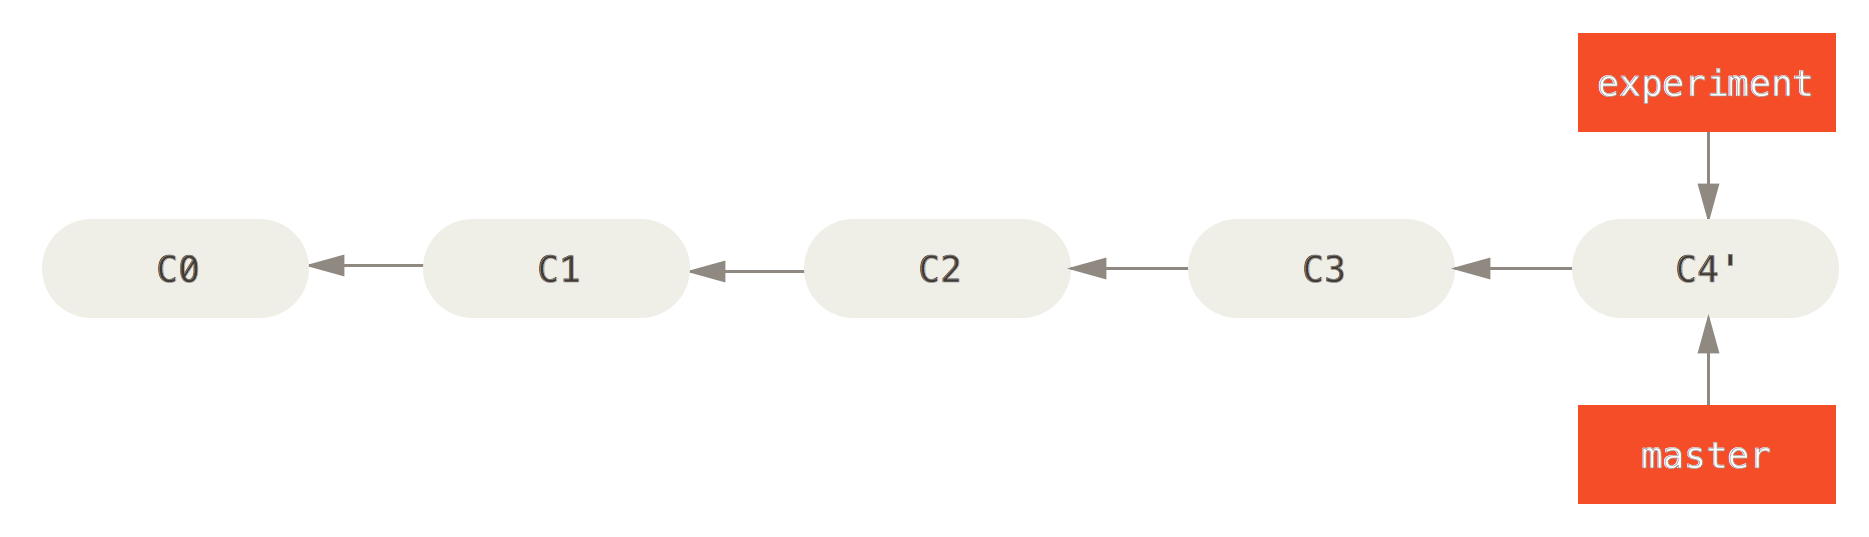
\includegraphics[height=3cm]{basic-rebase-4.png}
  \end{block}

\end{frame}


% tagging

\begin{frame}[fragile]
  \frametitle{tagging}
  Tags are good ways to mark commits. Also useful for people when they checkout your code. 

  \begin{lstlisting}[caption=tagging] 
   git tag
   git tag -a v1.4 -m "my version 1.4"
   git show v1.4
  \end{lstlisting}

  Can create lightweight tags (just the checksum) by not adding -a.

\end{frame}

% diffing

\begin{frame}[fragile]
  \frametitle{diff}
  Tools to see the differences and create patches from these differences.

  \begin{lstlisting}[caption=diff examples] 
   git diff
   git diff HEAD
   git diff HEAD^ HEAD
  \end{lstlisting}

  Various other tools like vimdiff, and more advanced diffs across branches

  \begin{lstlisting}[caption=diff examples 2] 
    git difftool --tool=vimdiff --no-prompt \
      origin/togusa:.vimrc .vimrc
  \end{lstlisting}

\end{frame}

% Flows

\begin{frame}
  \frametitle{Flows}
  A way to organise your work. Use branches and tags to keep work organised. 
 
  \begin{itemize}
    \item development/trunk
    \item stage/pre-production
    \item production/live
  \end{itemize}
 
\end{frame}

% Build Systems

\begin{frame}
  \frametitle{Integrating Git with workflow}
  Git and github work well with other tools. Automatic build-tools  

  \begin{itemize} 
    \item https://travis-ci.org/
    \item https://jenkins.io/index.html
  \end{itemize}
 
\end{frame}

% segue into testing

\begin{frame}
  \frametitle{Integrating Git with workflow 2}
  Can also automatically test code upon commit ... 

\end{frame}


\end{document}

